\section{Introduction}
\label{sec:introduction}

Language models first made intermediate computation visible through chain-of-thought prompting and self-consistency sampling~\citep{wei2022cot,wang2023selfconsistency}.
Agent benchmarks extend this trace to interleaved thoughts, tool calls, and environment feedback, as in ReAct and Toolformer-style tool use~\citep{yao2023react,schick2023toolformer}.
Yet most reports still collapse each rollout to one scalar: a pass/fail label, reward score, or leaderboard average.
Such scores rank systems, but they do not reveal what process a benchmark rewards.

\begin{figure}[t]
\centering
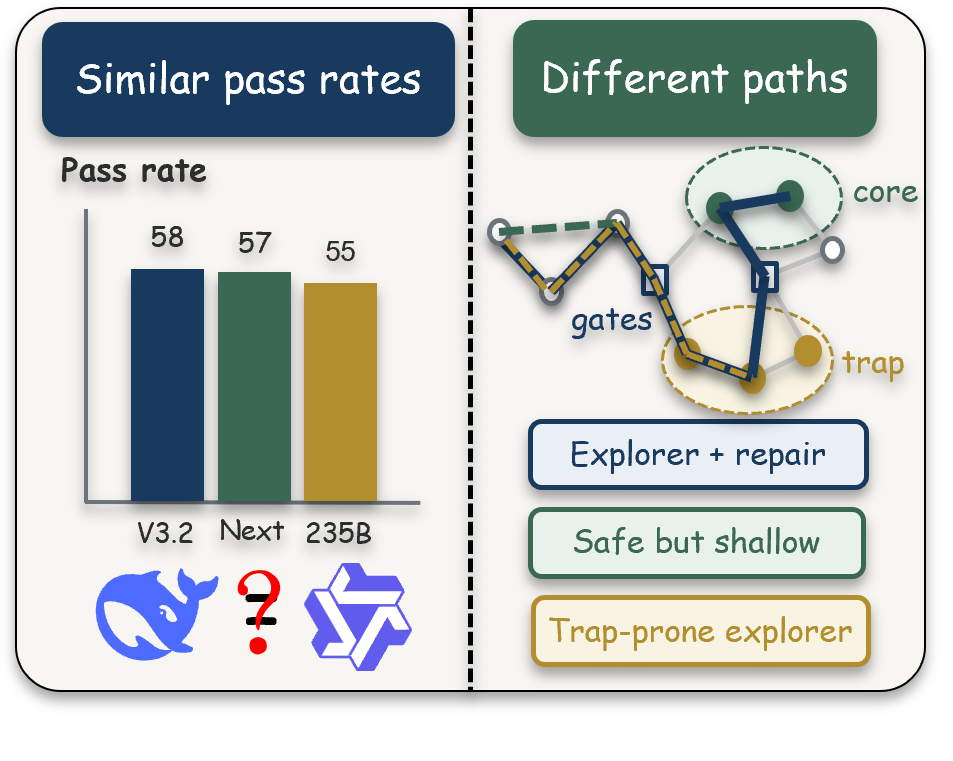
\includegraphics[width=\columnwidth]{figures/teaser.png}
\caption{Pass rates can hide process diversity. \textbf{Left}: three models score within 3 points on the same benchmark. \textbf{Right}: on a shared decision landscape built from pooled rollouts, they follow distinct paths: broad exploration with repair, shallow trap avoidance, or high-access navigation with more trap exposure.}
\label{fig:teaser}
\end{figure}

The challenge is that these process differences are not exposed as aligned units. Agent trajectories are long, branching, and benchmark-specific; their states mix tool choices, observations, file cues, environment feedback, and partial evidence. A single rollout can be inspected manually, but such inspection does not tell us whether another model reached an analogous state, avoided the same failure region, or recovered through a different route. What is missing is a shared coordinate system for comparing many trajectories as movements through the same task landscape.

We introduce \method{}, a framework that analyzes agent behavior not by inspecting individual trajectories in isolation, but by placing many trajectories from different models onto a shared graph-based decision landscape using observable action-observation signatures. The key hypothesis is that, once trajectories are aligned through observable action–observation states, model behaviors are not arbitrary traces: they form recurring traffic patterns over task-specific regions. 
\method{} then overlays outcome-informed productive cores and trap regions, and summarizes each rollout with three events: reaching a core (\emph{Access}), entering a trap (\emph{Trap exposure}), and returning from a trap to a core (\emph{Repair}).
The name reflects the workflow: traces become graphs, and models are compared by how they move through the resulting landscape.
These roles use terminal outcomes by design, so \method{} is descriptive rather than a blind success predictor: given a common map, what process does each model supply, and what process does each benchmark demand?

A shared landscape is useful not only for retrospective diagnosis, but also for deciding when a live agent trajectory has entered a historically risky region.
If trap regions correspond to repeatable trajectory states, an online detector built from those states should identify moments where a small recovery policy can help.
We therefore instantiate a \method{}-guided trap-aware prefix-fork pipeline on the benchmark with the clearest positive Repair demand.
An agent proceeds until a trap detector fires; matched continuations then resume from the same state while varying a conservative diagnosis note and a temperature bump.
The goal is not to claim a universal recovery mechanism, but to show that graph-derived traps can guide a downstream policy that improves task resolution.

Our contributions can be summarized:
\begin{itemize}
% \end{itemize}[leftmargin=*,itemsep=0.15em]
\item \textbf{\method{} for shared decision landscapes.}
We construct model-agnostic task graphs from pooled rollouts, then overlay outcome-informed core and trap regions after graph construction.
\item \textbf{A compact process profile.}
Across a five-split trajectory release spanning 7,329 records, 427 tasks, and five models, Access, Trap exposure, and Repair separate model navigation styles and benchmark demands that aggregate scores collapse.
\item \textbf{A \method{}-guided recovery pipeline.}
Because \swe{} shows the clearest positive Repair demand, we turn graph-derived traps into runtime triggers and test two single-factor recovery policies on all 500 \swe{} Verified instances. The best pooled policy improves resolved rate by $+3.1$ points ($p{=}0.016$) on the per-provider fired subset and by $+3.8$ points ($p{=}0.045$) on common-fired instances, while the active component differs by provider.
\end{itemize}
% \end{enumerate}
